\begin{problem}
  Repeat problem 2 with the basis $\{ \sin(j\pi x)\}$.
\end{problem}

\begin{proof}
  We use the same methods outlined in the solution to problem 2 to obtain an
  approximation using the basis $\{\phi_j(x) \}$ with $\phi_j(x) = \sin(j\pi x)$.
  Now we see see that,
  \begin{align*}
    \phi_j'(x)
    &= j\pi \cos(j\pi x)
  \end{align*}
  for $j=1,\dots,n$.

  Using the MATLAB function $\texttt{approximation.m}$, we construct the above
  system of equations and solve them arriving at approximations to the exact
  solution for $n=2,3,4$.
  The tables comparing the exact solution to these approximations at the
  points $x=0.25, 0.50, 0.75$ can be found below.

  \begin{table}[h!]
    \centering
    \bgroup
    \def\arraystretch{1.75}
    \begin{tabular}{| l | c | c | c | c |}
      \hline
      $x$ & $y(x)$ & $y_{2}(x)$ & $|y(x) - y_{2}(x)|$ & \pbox{5cm}{$\frac{100|y(x) - y_{2}(x)|}{|y(x)|}$} \\
      \hline
      0.25 & 3.504760e-02 & 3.355071e-02 & 1.496893e-03 & 4.271028 \\
      0.50 & 5.659056e-02 & 5.856881e-02 & 1.978250e-03 & 3.495724 \\
      0.75 & 5.027579e-02 & 4.927810e-02 & 9.976905e-04 & 1.984435 \\
      \hline
    \end{tabular}
    \egroup
    \caption{Comparison of approximation $y_{2}$ to solution $y$ using basis $\phi_j = \sin(j\pi x)$. All computations are rounded to 6 significant digits.}
  \end{table}

  \begin{table}[h!]
    \centering
    \bgroup
    \def\arraystretch{1.75}
    \begin{tabular}{| l | c | c | c | c |}
      \hline
      $x$ & $y(x)$ & $y_{3}(x)$ & $|y(x) - y_{3}(x)|$ & \pbox{5cm}{$\frac{100|y(x) - y_{3}(x)|}{|y(x)|}$} \\
      \hline
      0.25 & 3.504760e-02 & 3.522118e-02 & 1.735810e-04 & 0.495272 \\
      0.50 & 5.659056e-02 & 5.620640e-02 & 3.841569e-04 & 0.678836 \\
      0.75 & 5.027579e-02 & 5.094857e-02 & 6.727834e-04 & 1.338186 \\
      \hline
    \end{tabular}
    \egroup
    \caption{Comparison of approximation $y_{3}$ to solution $y$ using basis $\phi_j = \sin(j\pi x)$. All computations are rounded to 6 significant digits.}
  \end{table}

  \begin{table}[!h]
    \centering
    \bgroup
    \def\arraystretch{1.75}
    \begin{tabular}{| l | c | c | c | c |}
      \hline
      $x$ & $y(x)$ & $y_{4}(x)$ & $|y(x) - y_{4}(x)|$ & \pbox{5cm}{$\frac{100|y(x) - y_{4}(x)|}{|y(x)|}$} \\
      \hline
      0.25 & 3.504760e-02 & 3.522118e-02 & 1.735810e-04 & 0.495272 \\
      0.50 & 5.659056e-02 & 5.620640e-02 & 3.841569e-04 & 0.678836 \\
      0.75 & 5.027579e-02 & 5.094857e-02 & 6.727834e-04 & 1.338186 \\
      \hline
    \end{tabular}
    \egroup
    \caption{Comparison of approximation $y_{4}$ to solution $y$ using basis $\phi_j = \sin(j\pi x)$. All computations are rounded to 6 significant digits.}
  \end{table}


  We also provide the graphs of these comparisons in Figure \ref{trig_plot}.

  \begin{figure}[h!]
    \begin{center}
      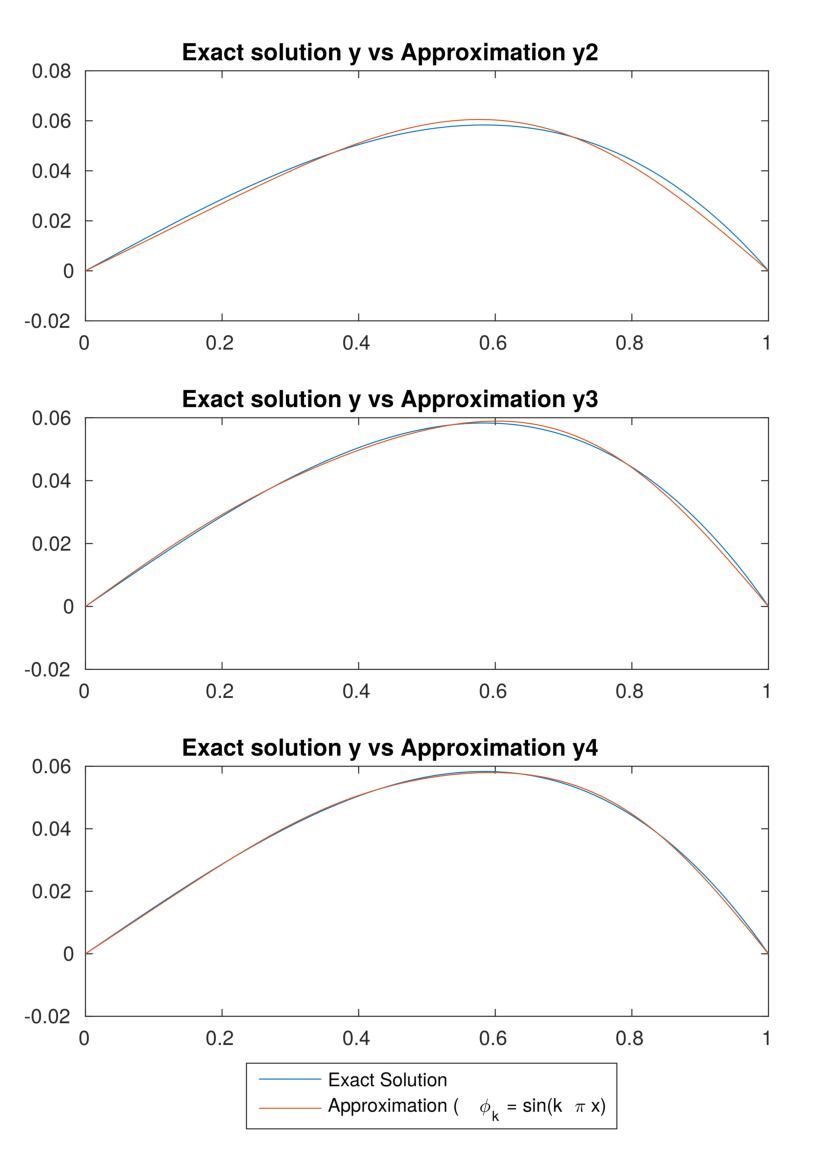
\includegraphics[scale=1.0]{trigonometric_basis_comparison}
    \end{center}
    \caption{Plots of exact solution $y$ and approximation $y_n$ over the interval $[0, 1]$
      using basis $\phi_j = \sin(j\pi x)$.}\label{trig_plot}
  \end{figure}

  The first value of $n$ such that the relative error of the approximation at
  each of the points $x_0=0.25, x_1=0.50, x_2=0.75$ is less than 5.0e-01\% is given by $n=6$.
  The relative errors $r_{x_i}$ at the above points for the approximation $y_6$ are
  $r_{x_0}$ = 3.080284e-01\%, $r_{x_1}$ = 2.293399e-01\%, and $r_{x_2}=$ 2.304205e-02\%.
  This value of $n$ needed for the relative error percents to be less than 5.0e-01\% is quite low.

  The general method of computing the coefficients suits our needs well enough
  if the goal is to obtain an approximation with a relative error less than 5.0e-01\% at these points.
  It will be mentioned, however, that the entries $a_{ij}$ of the coefficient matrix
  found in \eqref{system_imp} admit a special structure due to the choice of basis.
  Namely,
  \begin{align*}
    a_{ij} =
    \begin{cases}
      0 & \text{if $i \neq j$} \\
      \frac{-j^2\pi^2}{2} - \frac{1}{2} & \text{if $i = j$} \\
    \end{cases}
  \end{align*}

  This suggests that the coefficient matrix is actually a diagonal matrix. Finding
  the solution to the system \eqref{system_imp} is therefore trivial and reduces
  the computational complexity of finding the approximation immensely as we only need
  to compute the entries of the coefficient matrix along the diagonal and the entries
  of the column vector in the system.

  In order to accommodate this special structure we have created conditional creations
  of the coefficient matrices in the code mentioned earlier.
\end{proof}
